% ==========================================================================
% INFO 4617 Web Data Science -- Week 9: Extracting Data from PDFs (Chapter 9)
% Build:  TEXINPUTS=../common: BIBINPUTS=../common: latexmk -pdf slides.tex
% (or run `make` from the slides/ directory)
% ==========================================================================
\documentclass[9pt,aspectratio=169]{beamer}
% Resolve the shared theme/preamble in ../common/ when compiling this
% file directly from its own folder (no TEXINPUTS needed).
\makeatletter\def\input@path{{../common/}}\makeatother
% ==========================================================================
% Shared preamble for INFO 4617 Web Data Science weekly lecture decks
% Based on the Gotham beamer theme (vendored in this directory).
% Each week's slides.tex does:  % ==========================================================================
% Shared preamble for INFO 4617 Web Data Science weekly lecture decks
% Based on the Gotham beamer theme (vendored in this directory).
% Each week's slides.tex does:  % ==========================================================================
% Shared preamble for INFO 4617 Web Data Science weekly lecture decks
% Based on the Gotham beamer theme (vendored in this directory).
% Each week's slides.tex does:  \input{preamble}  (with common/ on TEXINPUTS)
% then sets \title/\subtitle/\author/\date and \begin{document}.
% ==========================================================================

\usetheme{gotham}

\usepackage{fbb}
\usepackage{booktabs}
\usepackage{graphicx}
\usepackage{tikz}
\usepackage{xcolor}
\usepackage{multirow}
\usepackage{listings}
\usetikzlibrary{positioning, arrows.meta, shapes}

% Bibliography
\usepackage[style=authoryear,
            backend=biber,
            maxcitenames=1,
            uniquename=false,
            uniquelist=false]{biblatex}
\addbibresource{bibliography.bib}

\gothamset{sectiontocframe default=off}

% ------------------------------------------------------------------ colors
\definecolor{cugold}{HTML}{CFB87C}
\definecolor{tab-red}{HTML}{E15759}
\definecolor{tab-orange}{HTML}{F28E2B}
\definecolor{tab-blue}{HTML}{4E79A7}
\definecolor{tab-cyan}{HTML}{76B7B2}
\definecolor{tab-green}{HTML}{59A14F}
\definecolor{tab-yellow}{HTML}{EDC948}
\definecolor{tab-purple}{HTML}{B07AA1}
\definecolor{tab-pink}{HTML}{FF9DA7}
\definecolor{tab-brown}{HTML}{9C755F}
\definecolor{tab-gray}{HTML}{BAB0AC}

\setbeamercolor{frametitle}{fg=black, bg=cugold}
\setbeamercolor{progress bar}{fg=cugold, bg=cugold!20}

\setbeamercolor{block title alerted}{fg=black, bg=cugold}
\setbeamercolor{block body alerted}{fg=black, bg=cugold!10}

% ------------------------------------------------------------------ footline
\setbeamertemplate{footline}{
  \begin{beamercolorbox}[wd=\paperwidth,ht=2.5ex,dp=1ex,right]{footline}
    {\footnotesize \insertframenumber{} of \inserttotalframenumber}
    \hspace*{2ex}
  \end{beamercolorbox}
}

% ------------------------------------------------------------------ helpers
\newcommand{\bottomcite}[1]{
    \vspace*{\fill}
    \vspace{-\baselineskip}
    {\tiny
    \rule{\textwidth}{0.3pt}\\
    #1
    }
    \vspace{0.5ex}
}

% Consistent code styling for the Wednesday "applied notebook" frames.
\lstdefinestyle{wds}{
    basicstyle=\ttfamily\scriptsize,
    keywordstyle=\color{tab-blue}\bfseries,
    commentstyle=\color{tab-green},
    stringstyle=\color{tab-orange},
    showstringspaces=false,
    breaklines=true,
    columns=fullflexible,
    language=Python,
    aboveskip=0.4em,
    belowskip=0.4em,
}
\lstset{style=wds}

% \dayband{Day}{Topic} -- a lightweight section divider label used to mark
% Monday / Wednesday / Friday within a week's deck.
\newcommand{\dayband}[2]{{\large\textbf{#1}}\;\textcolor{tab-gray}{\textbar}\;#2}
  (with common/ on TEXINPUTS)
% then sets \title/\subtitle/\author/\date and \begin{document}.
% ==========================================================================

\usetheme{gotham}

\usepackage{fbb}
\usepackage{booktabs}
\usepackage{graphicx}
\usepackage{tikz}
\usepackage{xcolor}
\usepackage{multirow}
\usepackage{listings}
\usetikzlibrary{positioning, arrows.meta, shapes}

% Bibliography
\usepackage[style=authoryear,
            backend=biber,
            maxcitenames=1,
            uniquename=false,
            uniquelist=false]{biblatex}
\addbibresource{bibliography.bib}

\gothamset{sectiontocframe default=off}

% ------------------------------------------------------------------ colors
\definecolor{cugold}{HTML}{CFB87C}
\definecolor{tab-red}{HTML}{E15759}
\definecolor{tab-orange}{HTML}{F28E2B}
\definecolor{tab-blue}{HTML}{4E79A7}
\definecolor{tab-cyan}{HTML}{76B7B2}
\definecolor{tab-green}{HTML}{59A14F}
\definecolor{tab-yellow}{HTML}{EDC948}
\definecolor{tab-purple}{HTML}{B07AA1}
\definecolor{tab-pink}{HTML}{FF9DA7}
\definecolor{tab-brown}{HTML}{9C755F}
\definecolor{tab-gray}{HTML}{BAB0AC}

\setbeamercolor{frametitle}{fg=black, bg=cugold}
\setbeamercolor{progress bar}{fg=cugold, bg=cugold!20}

\setbeamercolor{block title alerted}{fg=black, bg=cugold}
\setbeamercolor{block body alerted}{fg=black, bg=cugold!10}

% ------------------------------------------------------------------ footline
\setbeamertemplate{footline}{
  \begin{beamercolorbox}[wd=\paperwidth,ht=2.5ex,dp=1ex,right]{footline}
    {\footnotesize \insertframenumber{} of \inserttotalframenumber}
    \hspace*{2ex}
  \end{beamercolorbox}
}

% ------------------------------------------------------------------ helpers
\newcommand{\bottomcite}[1]{
    \vspace*{\fill}
    \vspace{-\baselineskip}
    {\tiny
    \rule{\textwidth}{0.3pt}\\
    #1
    }
    \vspace{0.5ex}
}

% Consistent code styling for the Wednesday "applied notebook" frames.
\lstdefinestyle{wds}{
    basicstyle=\ttfamily\scriptsize,
    keywordstyle=\color{tab-blue}\bfseries,
    commentstyle=\color{tab-green},
    stringstyle=\color{tab-orange},
    showstringspaces=false,
    breaklines=true,
    columns=fullflexible,
    language=Python,
    aboveskip=0.4em,
    belowskip=0.4em,
}
\lstset{style=wds}

% \dayband{Day}{Topic} -- a lightweight section divider label used to mark
% Monday / Wednesday / Friday within a week's deck.
\newcommand{\dayband}[2]{{\large\textbf{#1}}\;\textcolor{tab-gray}{\textbar}\;#2}
  (with common/ on TEXINPUTS)
% then sets \title/\subtitle/\author/\date and \begin{document}.
% ==========================================================================

\usetheme{gotham}

\usepackage{fbb}
\usepackage{booktabs}
\usepackage{graphicx}
\usepackage{tikz}
\usepackage{xcolor}
\usepackage{multirow}
\usepackage{listings}
\usetikzlibrary{positioning, arrows.meta, shapes}

% Bibliography
\usepackage[style=authoryear,
            backend=biber,
            maxcitenames=1,
            uniquename=false,
            uniquelist=false]{biblatex}
\addbibresource{bibliography.bib}

\gothamset{sectiontocframe default=off}

% ------------------------------------------------------------------ colors
\definecolor{cugold}{HTML}{CFB87C}
\definecolor{tab-red}{HTML}{E15759}
\definecolor{tab-orange}{HTML}{F28E2B}
\definecolor{tab-blue}{HTML}{4E79A7}
\definecolor{tab-cyan}{HTML}{76B7B2}
\definecolor{tab-green}{HTML}{59A14F}
\definecolor{tab-yellow}{HTML}{EDC948}
\definecolor{tab-purple}{HTML}{B07AA1}
\definecolor{tab-pink}{HTML}{FF9DA7}
\definecolor{tab-brown}{HTML}{9C755F}
\definecolor{tab-gray}{HTML}{BAB0AC}

\setbeamercolor{frametitle}{fg=black, bg=cugold}
\setbeamercolor{progress bar}{fg=cugold, bg=cugold!20}

\setbeamercolor{block title alerted}{fg=black, bg=cugold}
\setbeamercolor{block body alerted}{fg=black, bg=cugold!10}

% ------------------------------------------------------------------ footline
\setbeamertemplate{footline}{
  \begin{beamercolorbox}[wd=\paperwidth,ht=2.5ex,dp=1ex,right]{footline}
    {\footnotesize \insertframenumber{} of \inserttotalframenumber}
    \hspace*{2ex}
  \end{beamercolorbox}
}

% ------------------------------------------------------------------ helpers
\newcommand{\bottomcite}[1]{
    \vspace*{\fill}
    \vspace{-\baselineskip}
    {\tiny
    \rule{\textwidth}{0.3pt}\\
    #1
    }
    \vspace{0.5ex}
}

% Consistent code styling for the Wednesday "applied notebook" frames.
\lstdefinestyle{wds}{
    basicstyle=\ttfamily\scriptsize,
    keywordstyle=\color{tab-blue}\bfseries,
    commentstyle=\color{tab-green},
    stringstyle=\color{tab-orange},
    showstringspaces=false,
    breaklines=true,
    columns=fullflexible,
    language=Python,
    aboveskip=0.4em,
    belowskip=0.4em,
}
\lstset{style=wds}

% \dayband{Day}{Topic} -- a lightweight section divider label used to mark
% Monday / Wednesday / Friday within a week's deck.
\newcommand{\dayband}[2]{{\large\textbf{#1}}\;\textcolor{tab-gray}{\textbar}\;#2}


\title[Week 9 · PDFs]{{\Huge Extracting Data from PDFs}}
\subtitle{Week 9 · Documents module · Textbook Chapter 9}
\author[Keegan]{\textbf{Brian C. Keegan, Ph.D.} \\ Associate Professor, Department of Information Science \\ University of Colorado Boulder}
\date{October 12, 14 \& 16, 2026}

\begin{document}

\maketitle

% -------------------------------------------------------------------------
\begin{frame}{This week at a glance}
    \begin{columns}[T]
        \begin{column}{0.62\textwidth}
            PDFs are the web's filing cabinets. This week we pry official records out of them and turn locked documents into data.

            \vspace{1em}

            \dayband{Monday}{Concepts \& notebook intro}
            \begin{itemize}\small
                \item Why PDFs resist extraction; reconstruction vs.\ reading
            \end{itemize}

            \vspace{0.5em}

            \dayband{Wednesday}{Notebook lab}
            \begin{itemize}\small
                \item Work the Chapter 9 notebook: PyPDF, regex cleanup, Boulder City Council minutes
            \end{itemize}

            \vspace{0.5em}

            \dayband{Friday}{Textbook revisions}
            \begin{itemize}\small
                \item Propose \& peer-review pull requests improving Chapter 9
            \end{itemize}
        \end{column}
        \begin{column}{0.34\textwidth}
            \begin{block}{Companion notebook}
                \footnotesize \texttt{ch-09-pdfs.ipynb}
            \end{block}
            \begin{alertblock}{Bring a laptop}
                \footnotesize Wednesday is hands-on --- we extract and debug live.
            \end{alertblock}
        \end{column}
    \end{columns}
\end{frame}

% =========================================================================
\section{Monday · Concepts}
% =========================================================================

\begin{frame}{The web's filing cabinets}
    \begin{columns}[T]
        \begin{column}{0.58\textwidth}
            PDFs are everywhere in institutional record-keeping: council minutes, bill texts, financial reports, court filings, academic papers, environmental impact assessments.

            \vspace{1em}

            They are the format of choice for ``official'' documents because they \textbf{preserve visual layout} across any device or printer. But that priority --- visual fidelity over semantic structure --- makes them \textbf{hostile to programmatic extraction}.

            \vspace{1em}

            The records locked inside are \textit{readymade} data (\textcite{salganik2018bit}): created for administration, not research, yet repurposable --- with effort --- to answer questions their creators never anticipated.
        \end{column}
        \begin{column}{0.38\textwidth}
            \centering
            
\includegraphics[width=\textwidth]{img/council_minutes_pdf.png}\\
            {\scriptsize Boulder City Council minutes --- our target this week.}
        \end{column}
    \end{columns}
    \bottomcite{Textbook Ch.~9, ``The Web's Filing Cabinets.''}
\end{frame}

\begin{frame}{A computer never reads a PDF}
    \begin{columns}[T]
        \begin{column}{0.56\textwidth}
            When \textbf{you} read a PDF you see paragraphs, tables, headers, and page numbers.

            \vspace{1em}

            When a \textbf{computer} reads one it sees a sequence of drawing instructions: \textit{place this character at $(x, y)$; draw a line from here to there; embed this image}.

            \vspace{1em}

            So text extraction is \textbf{reconstruction, not reading} --- the computer must infer logical structure from spatial layout. The results will not be perfect, but they can be good enough to turn inaccessible records into analyzable datasets.
        \end{column}
        \begin{column}{0.4\textwidth}
            \centering
            
\includegraphics[width=\textwidth]{img/pdf_drawing_instructions.png}\\
            {\scriptsize Glyphs at coordinates, not sentences --- structure is inferred.}
        \end{column}
    \end{columns}
    \bottomcite{Textbook Ch.~9, ``The Web's Filing Cabinets.''}
\end{frame}

\begin{frame}{Soft enclosure \& the infrastructure of transparency}
    \begin{columns}[T]
        \begin{column}{0.58\textwidth}
            When governments publish minutes, budgets, and filings \textit{only} as PDFs, they create what the book's post-API chapter calls \textbf{soft enclosure}: records that are nominally public but practically inaccessible for analysis.

            \vspace{0.75em}

            Building extraction skills enacts the \textbf{oversight} and \textbf{ownership} values --- public records belong to the public, and technical barriers are themselves a form of enclosure.

            \vspace{0.75em}

            Adobe created the PDF in 1993 for visual fidelity across devices --- at the cost of semantic accessibility. \textbf{DocumentCloud} (ProPublica \& IRE), \textbf{MuckRock} (automating FOIA), and the \textbf{Sunlight Foundation} built the infrastructure that bridges public documents and accessible data.
        \end{column}
        \begin{column}{0.38\textwidth}
            \centering
            
\includegraphics[width=\textwidth]{img/documentcloud.png}\\
            {\scriptsize DocumentCloud: shared infrastructure for analyzing document dumps.}
        \end{column}
    \end{columns}
    \bottomcite{Textbook Ch.~9, ``Public Interest Connection'' \& ``Social History and Public Interest.''}
\end{frame}

\begin{frame}{What the notebook covers}
    This week's companion notebook builds one skill at a time:
    \begin{itemize}
        \item \textbf{PyPDF basics} --- open a file, read metadata, extract page-level text (and see how messy it is)
        \item \textbf{Cleanup} --- normalize whitespace \textit{without} destroying line structure; use regex to impose fields
        \item \textbf{Case study} --- Boulder City Council minutes: council attendance and public-comment counts
        \item \textbf{Pipeline} --- a reusable class that processes a whole corpus of PDFs into a DataFrame
    \end{itemize}

    \vspace{0.75em}

    \begin{alertblock}{Connecting to Ch.~7 \& the post-API theme}
        \footnotesize Once text is out, the \textbf{bag-of-words} preprocessing from the archives chapter (Ch.~7) sharpens topic tracking across many meetings. And PDF-only publishing \textit{is} the ``soft enclosure'' the post-API chapter warns about --- extraction is how we push back.
    \end{alertblock}
\end{frame}

% =========================================================================
\section{Wednesday · Notebook Lab}
% =========================================================================

\begin{frame}[fragile]{PyPDF basics --- open, inspect, extract}
    \texttt{pypdf} gives you document metadata and page-level text. Start by looking at what actually comes out:
\begin{lstlisting}
from pypdf import PdfReader

reader = PdfReader("council_minutes_2024_01.pdf")
print(len(reader.pages), "pages")
print(reader.metadata)                 # title, author, creation date...

page = reader.pages[0]
text = page.extract_text()
print(text[:500])   # expect mess: headers/footers mixed in, tables garbled,
                    # line breaks that don't match paragraphs
\end{lstlisting}
    \bottomcite{Textbook Ch.~9, ``PyPDF Basics.'' Messy output is normal --- cleaning it up is the core of the workflow.}
\end{frame}

\begin{frame}[fragile]{The one line that flattens the page}
    \begin{columns}[T]
        \begin{column}{0.54\textwidth}
        Tempting one-liner:
\begin{lstlisting}
# DON'T: \s matches newlines too,
# so this flattens the whole page
re.sub(r'\s+', ' ', raw_text)
\end{lstlisting}
        Correct --- collapse spaces \& tabs, \textbf{keep} the line breaks:
\begin{lstlisting}
text = re.sub(r'[ \t]+', ' ', raw_text)
lines = [ln.strip() for ln in text.split('\n')]
clean = '\n'.join(ln for ln in lines if ln)
\end{lstlisting}
        \end{column}
        \begin{column}{0.44\textwidth}
            The most important choice is what \textit{not} to collapse.

            \vspace{0.75em}

            Line structure is real information: section headings are recognizable \textbf{precisely because they sit alone on their own lines}.

            \vspace{0.75em}

            Erase the newlines and no heading detector can ever find them.
        \end{column}
    \end{columns}
    \bottomcite{Textbook Ch.~9, ``Cleanup Strategies.''}
\end{frame}

\begin{frame}[fragile]{A regex toolkit for PDF text}
    Structured data hides inside a wall of characters; regex carves it out. Five patterns cover most government PDFs:
\begin{lstlisting}
dates    = re.findall(r'\d{1,2}/\d{1,2}/\d{2,4}', text)     # 1/15/2024, 12/03/23
amounts  = re.findall(r'\$[\d,]+\.?\d*', text)              # $1,250.00, $3,400,000
emails   = re.findall(r'[\w.+-]+@[\w-]+\.[\w.-]+', text)    # clerk@bouldercolorado.gov

# ALL-CAPS section headings on their own line (a literal space, NOT \s,
# so one match can't swallow several consecutive heading lines):
headings = re.findall(r'^[A-Z][A-Z0-9 .:&-]{5,}$', text, re.MULTILINE)
# -> ['CALL TO ORDER', 'PUBLIC COMMENT', 'CONSENT AGENDA', 'ADJOURNMENT']
\end{lstlisting}
    Each pattern encodes an assumption (slash dates, a leading \texttt{\$}, uppercase headings). \textbf{Test across multiple pages and documents} before trusting a pipeline. New to regex? See \textit{Missing Manual} Ch.~18.
    \bottomcite{Textbook Ch.~9, ``Regular Expressions for PDF Text.''}
\end{frame}

\begin{frame}[fragile]{Case study --- council attendance}
    \begin{columns}[T]
        \begin{column}{0.58\textwidth}
\begin{lstlisting}
def extract_attendance(pdf_path):
    text = PdfReader(pdf_path).pages[0].extract_text()
    # names follow "Present:" up to "Absent:" or end of line
    present = re.search(r'Present:\s*(.*?)\s*(?:Absent:|$)',
                        text, re.IGNORECASE | re.MULTILINE)
    absent  = re.search(r'Absent:\s*(.*)$',
                        text, re.IGNORECASE | re.MULTILINE)
    return {"present": split_names(present),
            "absent":  split_names(absent)}
\end{lstlisting}
        \end{column}
        \begin{column}{0.4\textwidth}
            \centering
            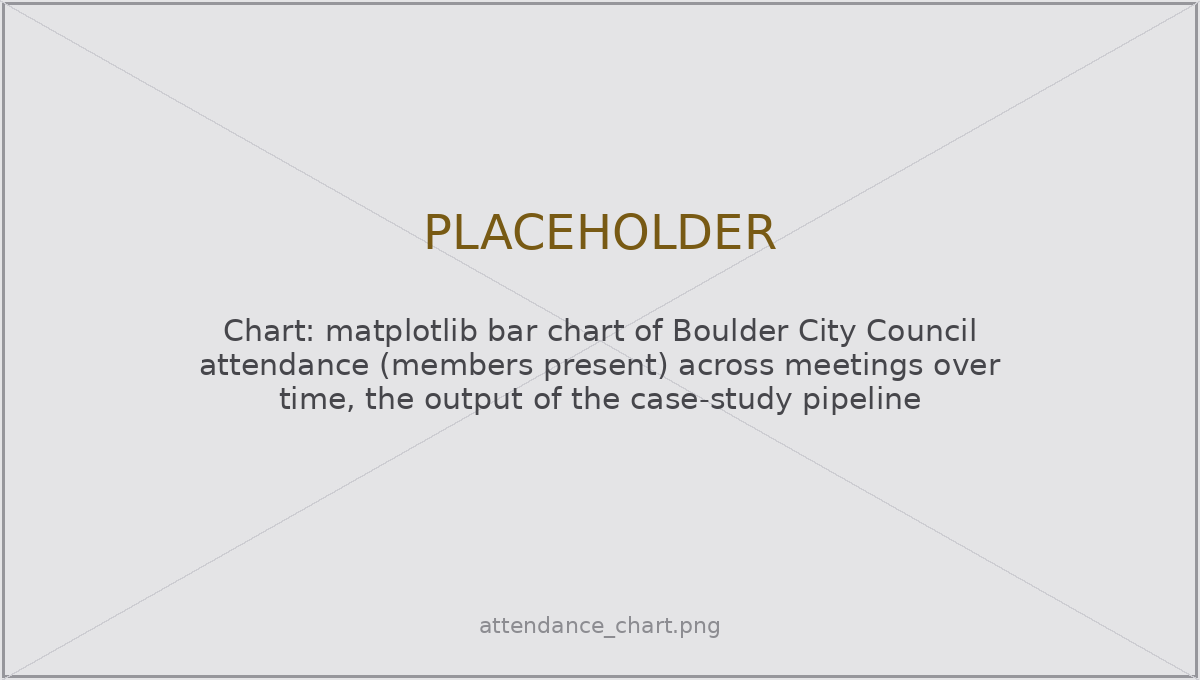
\includegraphics[width=\textwidth]{img/attendance_chart.png}\\
            {\scriptsize Counts across meetings become a trend --- scale reveals what one PDF can't.}
        \end{column}
    \end{columns}
    \vspace{0.3em}
    {\small Be honest about limits: ``Absent: None'' becomes a phantom member named \texttt{None}; titles and separators vary. Treat output as a \textbf{first draft} --- spot-check and patch.}
    \bottomcite{Textbook Ch.~9, ``Case Study: Boulder City Council Minutes.'' Filenames encode the date --- parse them, not the PDF text.}
\end{frame}

\begin{frame}[fragile]{Scale it --- a reusable corpus pipeline}
    \begin{columns}[T]
        \begin{column}{0.6\textwidth}
        Wrap the workflow so one class processes a whole directory into a DataFrame:
\begin{lstlisting}
class PDFCorpusAnalyzer:
    def __init__(self, directory, cleanup_patterns=None):
        self.files = sorted(f for f in os.listdir(directory)
                            if f.lower().endswith(".pdf"))
        self.cleanup_patterns = cleanup_patterns or []

    def process_all(self, extract_fn):
        rows = []
        for f in self.files:
            try:                       # one bad PDF won't kill the run
                text = self.extract_text(f)
                rows.append({**extract_fn(f, text), "file": f})
            except Exception as e:
                rows.append({"file": f, "error": str(e)})
        return pd.DataFrame(rows)
\end{lstlisting}
        \end{column}
        \begin{column}{0.38\textwidth}
            \centering
            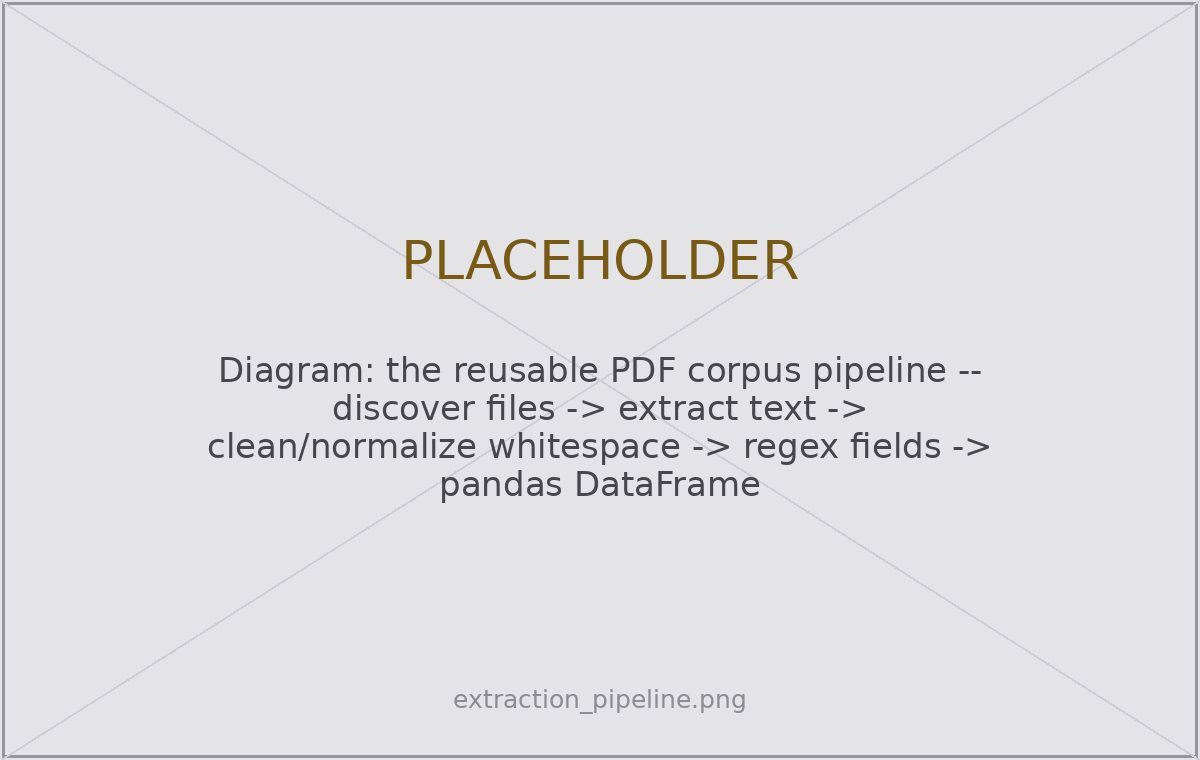
\includegraphics[width=\textwidth]{img/extraction_pipeline.png}\\
            {\scriptsize Discover $\rightarrow$ extract $\rightarrow$ clean $\rightarrow$ regex fields $\rightarrow$ DataFrame.}
        \end{column}
    \end{columns}
    \bottomcite{Textbook Ch.~9, ``Building a Reusable PDF Pipeline.'' Pass document-specific cleanup patterns in; wrap each file defensively.}
\end{frame}

\begin{frame}[fragile]{When PyPDF is not enough}
    PyPDF handles text-based PDFs well, but two common cases defeat it.

    \vspace{0.4em}
    \textbf{Tables} --- PyPDF flattens them into a text stream, losing rows and columns. \texttt{pdfplumber} preserves the grid:
\begin{lstlisting}
import pdfplumber
with pdfplumber.open("report.pdf") as pdf:
    table = pdf.pages[0].extract_table()   # a list of row-lists (cells)
    df = pd.DataFrame(table[1:], columns=table[0])
\end{lstlisting}
    \textbf{Scanned PDFs} --- a scan has no text layer, so PyPDF returns empty or garbled output. You need \textbf{OCR}:
\begin{lstlisting}
# pytesseract + the Tesseract engine turn page images into text;
# accuracy varies with scan quality. (camelot is another table option.)
\end{lstlisting}
    Know your tool's limits: reach for \texttt{pdfplumber}, \texttt{camelot}, or OCR when the layout demands it.
    \bottomcite{Textbook Ch.~9, ``When PyPDF Is Not Enough'' \& ``Common Issues to Debug.''}
\end{frame}

\begin{frame}{Lab: work these, then show-and-tell}
    \begin{columns}[T]
        \begin{column}{0.62\textwidth}
            Work through the notebook exercises in pairs:
            \begin{enumerate}\small
                \item Find \& extract one consistent element across $\geq 10$ government PDFs $\rightarrow$ a DataFrame
                \item Compare PyPDF quality on a text report, a table-heavy doc, and a slide deck
                \item Tables, not text: extract a budget table with \texttt{pdfplumber} vs.\ \texttt{pypdf}; build numeric columns
                \item Topic tracking: count a term (``housing,'' ``police,'' ``flood'') across a year of minutes; plot spikes (reuse Ch.~7 bag-of-words)
                \item Tool comparison: \texttt{pdfplumber} vs.\ \texttt{pypdf} on the same PDF
                \item[6.] \textcolor{tab-purple}{\textbf{5617}}: quantify extraction quality across two cities' PDFs; write a data-quality memo using \textcite{gebru2021datasheets} categories
            \end{enumerate}
        \end{column}
        \begin{column}{0.34\textwidth}
            \begin{block}{Show-and-Tell}
                \footnotesize Come ready to share:
                \begin{itemize}\footnotesize
                    \item a challenging bug
                    \item interesting data you pulled
                    \item a provocation for a research design
                \end{itemize}
            \end{block}
        \end{column}
    \end{columns}
\end{frame}

\begin{frame}[standout]
    PDFs are built for eyes, not for code.\\
    Every extraction is an educated reconstruction ---\\
    never perfect, often good enough.\\[1em]
    {\large Imprecision is the price of scale ---\\ and scale is what turns documents into data.}
\end{frame}

% =========================================================================
\section{Friday · Textbook Revisions}
% =========================================================================

\begin{frame}{Improving Chapter 9 together}
    \begin{columns}[T]
        \begin{column}{0.6\textwidth}
            Today we make the book better. Each of you opens a \textbf{pull request} against \texttt{ch-09-pdfs.qmd} and reviews a classmate's.

            \vspace{1em}

            The workflow (from Week 1):
            \begin{enumerate}\small
                \item Branch / fork the book repo
                \item Edit the chapter; commit with a clear message
                \item Open a PR describing \textit{what} and \textit{why}
                \item Review two peers' PRs: kind, specific, actionable
            \end{enumerate}
        \end{column}
        \begin{column}{0.36\textwidth}
            \centering
            
\includegraphics[width=\textwidth]{img/pr_review.png}
        \end{column}
    \end{columns}
    \bottomcite{Contributions \& reviews count toward the Textbook Revisions grade (30\%).}
\end{frame}

\begin{frame}{A revision menu for Chapter 9}
    High-value targets --- pick one and scope it to a single PR:
    \begin{itemize}
        \item \textbf{Run it against real Boulder minutes.} The \texttt{\# Returns:} outputs and five regex patterns are \textit{illustrative}. Download actual signed minutes, report what the patterns catch and miss, and label sample output as representative.
        \item \textbf{Add the chapter's first figures.} It is all code and prose today: a ``drawing-instructions vs.\ logical text'' diagram, a pipeline flowchart, or an annotated minutes screenshot would anchor Monday's core idea.
        \item \textbf{Harden \texttt{extract\_attendance}.} The chapter itself flags ``Absent: None,'' title variants (``Council Member Smith''), and semicolon / line-break separators. Contribute handling \textbf{plus tests} for the formats you actually hit.
        \item \textbf{Make an exercise self-checking.} Add expected output, a rubric, or a starter cell to the open-ended ``find and extract'' and ``topic tracking'' exercises.
        \item \textbf{Deepen ``When PyPDF Is Not Enough.''} Turn the two-line \texttt{pdfplumber} / OCR sketches into a runnable table-extraction or Tesseract example tied to ``Further Reading.''
    \end{itemize}
    \bottomcite{Targets drawn from the chapter's callouts, ``Common Issues,'' exercises, \& ``Further Reading.''}
\end{frame}

\begin{frame}{What makes a good revision \& a good review}
    \begin{columns}[T]
        \begin{column}{0.48\textwidth}
            \begin{block}{A strong PR}
                \begin{itemize}\small
                    \item One focused change, clearly titled
                    \item Explains the problem it fixes
                    \item Builds (\texttt{quarto render}) without errors
                    \item Matches the book's voice and notation
                    \item Discloses any AI assistance
                \end{itemize}
            \end{block}
        \end{column}
        \begin{column}{0.48\textwidth}
            \begin{block}{A strong review}
                \begin{itemize}\small
                    \item Runs / reads the change, not just skims
                    \item Names specifics (line, claim, code)
                    \item Separates ``must fix'' from ``nice to have''
                    \item Is generous --- assume good faith
                    \item Ends with a clear verdict
                \end{itemize}
            \end{block}
        \end{column}
    \end{columns}
    \vspace{0.5em}
    \centering\small Next week: a new module on \textbf{APIs} --- when data arrives as JSON and no parsing is required (starting with Wikipedia).
\end{frame}

% =========================================================================
\begin{frame}{Key takeaways}
    \begin{enumerate}
        \item PDFs optimize \textbf{visual fidelity over structure} --- extraction is reconstruction, not reading.
        \item \texttt{pypdf} gives page-level text \& metadata; expect messy output and plan to clean it.
        \item Collapse spaces/tabs but \textbf{keep newlines} --- line structure is information; regex imposes the rest.
        \item Abstract into a \textbf{pipeline} so one bad file doesn't kill a corpus run; test patterns across documents.
        \item Know PyPDF's limits: \texttt{pdfplumber} for tables, OCR for scans. Imprecision is the price of scale.
    \end{enumerate}
    \vspace{1em}
    \bottomcite{Reading: Textbook Ch.~9. Related: \textcite{salganik2018bit}; \textcite{gebru2021datasheets}.}
\end{frame}

\end{document}
